% Options for packages loaded elsewhere
\PassOptionsToPackage{unicode}{hyperref}
\PassOptionsToPackage{hyphens}{url}
\PassOptionsToPackage{dvipsnames,svgnames,x11names}{xcolor}
%
\documentclass[
  letterpaper,
  DIV=11,
  numbers=noendperiod]{scrartcl}

\usepackage{amsmath,amssymb}
\usepackage{iftex}
\ifPDFTeX
  \usepackage[T1]{fontenc}
  \usepackage[utf8]{inputenc}
  \usepackage{textcomp} % provide euro and other symbols
\else % if luatex or xetex
  \usepackage{unicode-math}
  \defaultfontfeatures{Scale=MatchLowercase}
  \defaultfontfeatures[\rmfamily]{Ligatures=TeX,Scale=1}
\fi
\usepackage{lmodern}
\ifPDFTeX\else  
    % xetex/luatex font selection
\fi
% Use upquote if available, for straight quotes in verbatim environments
\IfFileExists{upquote.sty}{\usepackage{upquote}}{}
\IfFileExists{microtype.sty}{% use microtype if available
  \usepackage[]{microtype}
  \UseMicrotypeSet[protrusion]{basicmath} % disable protrusion for tt fonts
}{}
\makeatletter
\@ifundefined{KOMAClassName}{% if non-KOMA class
  \IfFileExists{parskip.sty}{%
    \usepackage{parskip}
  }{% else
    \setlength{\parindent}{0pt}
    \setlength{\parskip}{6pt plus 2pt minus 1pt}}
}{% if KOMA class
  \KOMAoptions{parskip=half}}
\makeatother
\usepackage{xcolor}
\setlength{\emergencystretch}{3em} % prevent overfull lines
\setcounter{secnumdepth}{-\maxdimen} % remove section numbering
% Make \paragraph and \subparagraph free-standing
\ifx\paragraph\undefined\else
  \let\oldparagraph\paragraph
  \renewcommand{\paragraph}[1]{\oldparagraph{#1}\mbox{}}
\fi
\ifx\subparagraph\undefined\else
  \let\oldsubparagraph\subparagraph
  \renewcommand{\subparagraph}[1]{\oldsubparagraph{#1}\mbox{}}
\fi


\providecommand{\tightlist}{%
  \setlength{\itemsep}{0pt}\setlength{\parskip}{0pt}}\usepackage{longtable,booktabs,array}
\usepackage{calc} % for calculating minipage widths
% Correct order of tables after \paragraph or \subparagraph
\usepackage{etoolbox}
\makeatletter
\patchcmd\longtable{\par}{\if@noskipsec\mbox{}\fi\par}{}{}
\makeatother
% Allow footnotes in longtable head/foot
\IfFileExists{footnotehyper.sty}{\usepackage{footnotehyper}}{\usepackage{footnote}}
\makesavenoteenv{longtable}
\usepackage{graphicx}
\makeatletter
\def\maxwidth{\ifdim\Gin@nat@width>\linewidth\linewidth\else\Gin@nat@width\fi}
\def\maxheight{\ifdim\Gin@nat@height>\textheight\textheight\else\Gin@nat@height\fi}
\makeatother
% Scale images if necessary, so that they will not overflow the page
% margins by default, and it is still possible to overwrite the defaults
% using explicit options in \includegraphics[width, height, ...]{}
\setkeys{Gin}{width=\maxwidth,height=\maxheight,keepaspectratio}
% Set default figure placement to htbp
\makeatletter
\def\fps@figure{htbp}
\makeatother

\KOMAoption{captions}{tableheading}
\makeatletter
\makeatother
\makeatletter
\makeatother
\makeatletter
\@ifpackageloaded{caption}{}{\usepackage{caption}}
\AtBeginDocument{%
\ifdefined\contentsname
  \renewcommand*\contentsname{Table of contents}
\else
  \newcommand\contentsname{Table of contents}
\fi
\ifdefined\listfigurename
  \renewcommand*\listfigurename{List of Figures}
\else
  \newcommand\listfigurename{List of Figures}
\fi
\ifdefined\listtablename
  \renewcommand*\listtablename{List of Tables}
\else
  \newcommand\listtablename{List of Tables}
\fi
\ifdefined\figurename
  \renewcommand*\figurename{Figure}
\else
  \newcommand\figurename{Figure}
\fi
\ifdefined\tablename
  \renewcommand*\tablename{Table}
\else
  \newcommand\tablename{Table}
\fi
}
\@ifpackageloaded{float}{}{\usepackage{float}}
\floatstyle{ruled}
\@ifundefined{c@chapter}{\newfloat{codelisting}{h}{lop}}{\newfloat{codelisting}{h}{lop}[chapter]}
\floatname{codelisting}{Listing}
\newcommand*\listoflistings{\listof{codelisting}{List of Listings}}
\makeatother
\makeatletter
\@ifpackageloaded{caption}{}{\usepackage{caption}}
\@ifpackageloaded{subcaption}{}{\usepackage{subcaption}}
\makeatother
\makeatletter
\@ifpackageloaded{tcolorbox}{}{\usepackage[skins,breakable]{tcolorbox}}
\makeatother
\makeatletter
\@ifundefined{shadecolor}{\definecolor{shadecolor}{rgb}{.97, .97, .97}}
\makeatother
\makeatletter
\makeatother
\makeatletter
\makeatother
\ifLuaTeX
  \usepackage{selnolig}  % disable illegal ligatures
\fi
\IfFileExists{bookmark.sty}{\usepackage{bookmark}}{\usepackage{hyperref}}
\IfFileExists{xurl.sty}{\usepackage{xurl}}{} % add URL line breaks if available
\urlstyle{same} % disable monospaced font for URLs
\hypersetup{
  colorlinks=true,
  linkcolor={blue},
  filecolor={Maroon},
  citecolor={Blue},
  urlcolor={Blue},
  pdfcreator={LaTeX via pandoc}}

\author{}
\date{}

\begin{document}
\ifdefined\Shaded\renewenvironment{Shaded}{\begin{tcolorbox}[interior hidden, borderline west={3pt}{0pt}{shadecolor}, boxrule=0pt, sharp corners, enhanced, breakable, frame hidden]}{\end{tcolorbox}}\fi

\hypertarget{conclusions-and-future-work}{%
\section{Conclusions and Future
Work}\label{conclusions-and-future-work}}

\hypertarget{sec-conclusions}{%
\subsection{Conclusions}\label{sec-conclusions}}

\hypertarget{general-overview}{%
\subsubsection{General Overview}\label{general-overview}}

I started writing this thesis with one broad aim \(-\) to couple insect
odorant receptors with either a carbon nanotube or graphene field-effect
transistor for highly selective sensing in the vapour phase. Through
this process, I hoped to gain new physical insights into the transducer
and receptor elements used, through careful examination of the
biosensors which resulted from their coupling. At the end of this
investigation, three broad themes have emerged:

\begin{itemize}
\item
  Slight variations in transducer morphology have a substantial impact
  on biosensor sensitivity and power consumption.
\item
  Intrinsic transducer hysteresis leads to biosensor current drift,
  which can be modelled and corrected for when interpreting sensing
  data.
\item
  Surface contamination can affect transducer functionalisation and lead
  to significant variability in biosensor quality.
\end{itemize}

These findings and their relation to the goal of creating a reliable
biosensor for a vapour-phase detection system are each detailed in this
section.

\hypertarget{biosensor-performance-and-transducer-morphology}{%
\subsubsection{Biosensor Performance and Transducer
Morphology}\label{biosensor-performance-and-transducer-morphology}}

Carbon nanotube networks and graphene are used as the thin-film for
sensing field-effect transistors due to their highly sensitive surface.
Features present on each film were found to enhance or reduce the
sensitivity of the transistor in a low-power configuration. The process
used for randomly depositing carbon nanotubes influences multiple
aspects of the resulting network morphology, including the density and
homogeneity of the network, the diameter of bundled carbon nanotubes,
the level of doping present and the relative proportion of metallic to
semiconducting nanotubes. These variables were investigated atomic force
microscopy, Raman spectroscopy and electrical characterisation. Devices
with carbon nanotubes deposited using surfactant in the presence of
steam were found to have relatively dense and homogeneous networks which
gave rise to highly consistent electrical characteristics, desirable for
biosensor reproducibility and multiplexing. Carbon nanotube bundle
diameters were also much smaller in these networks, which gave them a
relatively large on-off ratio and subthreshold slope, figures of merit
which correspond to low power operation. However, steam-assisted
surfactant-deposited devices were found to have significant
\(p\)-doping. Identifying and removing the source of this \(p\)-doping
would further enhance the performance of these devices.

\hypertarget{biosensor-drift-and-transducer-hysteresis}{%
\subsubsection{Biosensor Drift and Transducer
Hysteresis}\label{biosensor-drift-and-transducer-hysteresis}}

All devices characterised showed a degree of hysteresis, which was
especially significant for solvent-deposited carbon nanotube network
devices as well as any device when backgated. This hysteresis is a
result of the evolving occupancy of charge traps, which are introduced
to the device by gate bias or adsorbed dopants. This changing occupancy
leads to a slow drift in current level when the transistor is operated
with constant voltages at both the drain and gate. If left until
reaching a steady state, this baseline drift can be modelled using a
linear combination of three exponentials. However, it is not feasible to
wait more than three hours for a biosensor to warm up with each use. A
series expansion was used to model the drift over a shorter period of
time, where the two longer time constant exponential terms were
approximated as linear. By waiting until the first exponential
approached zero, a simple linear correction was sufficient to filter out
baseline drift when the time constants of the other exponentials were
sufficiently large. For a pristine, liquid-gated steam-deposited carbon
nanotube device, the first exponential typically took less than 30
minutes to sufficiently decay.

\hypertarget{biosensor-functionalisation-and-transducer-contamination}{%
\subsubsection{Biosensor Functionalisation and Transducer
Contamination}\label{biosensor-functionalisation-and-transducer-contamination}}

While the pristine surfactant-deposited carbon nanotube transistors were
consistently sensitive to changes in both an aqueous and vapour
environment, their selective detection ability after non-covalent
functionalisation with iORs was highly variable. Using atomic force
microscopy, Raman spectroscopy, electrical characterisation and
fluorescence microscopy it was found that the PBASE linker was
successfully attaching iOR nanodiscs to the carbon nanotube network.
While functionalisation caused significant gating of the network for
devices which were successful sensors, it was not seen for devices which
showed no selective sensing behaviour, despite the evidence that iOR
nanodiscs were present in both cases. It was therefore hypothesised that
an unknown coating on the transducer was allowing the adhesion of iOR
nanodiscs onto the channel region, but was preventing electrical
interactions between iORs and the channel. A pristine thin-film device
with a thin surface coating can still be electrostatically or
capacitively gated in a highly sensitive manner. However, it has
previously been noted that the primary sensing mechanism of iORs appears
to be through direct charge transfer. If an insulating coating layer is
present, it may prevent charge from passing between the iORs and the
channel.

Multiple potential candidates for this unwanted coating were identified
throughout the course of this thesis, including residual process
chemicals, residual PBASE and hydrophobic alkanes. Sensing experiments
were then performed that systematically eliminated possible candidates.
It was found that neither avoiding the introduction of surfactant or
ensuring PBASE did not hydrolyse led to consistent biosensors. Finally,
a method was tested that eliminated the remaining possible candidates
through the use of a oxygen plasma clean step prior to
functionalisation, as well as the use of iORs in surfactant solution
with linker pre-attached. This process resulted in a successful sensor
in an aqueous environment, which is further indication that an unwanted
surface coating is the cause of sensor variability. It should be noted
that the impact of oxygen plasma on device mobility and the
vulnerability of the unprotected iORs means that this method does not
reliably produce responsive vapour-phase sensors. Further optimisation
of the functionalisation process is a clear priority for future works,
with a detailed discussion of possible approaches found in the next
section.

\hypertarget{sec-future-work}{%
\subsection{Future Work}\label{sec-future-work}}

\hypertarget{sec-future-work-fabrication}{%
\subsubsection{Device Fabrication and
Functionalisation}\label{sec-future-work-fabrication}}

Throughout the course of this thesis, several aspects of the fabrication
and functionalisation were identified as having potential for
improvement. Further investigation into these approaches by future
researchers could lead to improved biosensor performance and a deeper
understanding of the device physics of the sensor. The encapsulation of
device electrodes is critical for improving the performance of a device,
preventing gate leakage through the liquid-gate and avoiding modulation
of the electrode-channel Schottky barrier while sensing {[}@Lim2014;
@Albarghouthi2022; @Heller2008{]}. Albarghouthi \emph{et al.} outline an
alternative encapsulation approach which leads to very low gate leakage
currents which could be adapted for use with our sensing devices
{[}@Albarghouthi2022{]}. Here, a multilayered encapsulation with
HfO\(_2\), SU8 and PEG is used to encapsulated the device. The only
change to the existing process required is the addition of a patterning
step to leave the channel region exposed, similar to that seen in
\textbf{?@sec-encapsulation}. Furthermore, if a nonfluorescent SU8 was
used instead of SU8-2150 {[}@Vobornik2023{]}, devices could be
characterised with fluorescence microscopy after encapsulation, which
would be highly advantageous for verifying functionalisation. After
passivation with PEG, highly specific attachment of fluorescence-tagged
iORs could be verified in a similar manner to that used by Lee \emph{et
al.} directly prior to sensing {[}@Lee2012b{]}. If PEG passivation and
linker are deposited simultaneously, as in the approach by Filipiak
\emph{et al.} {[}@Filipiak2018{]}, multiplexed fluorescence microscopy
could be used to determine the proportion of channel coverage by linker
compared with PEG passivation.

Surface contamination was identified as one of the major factors
interfering with successful device functionalisation in this thesis. To
improve the reproducibility and yield of non-covalent functionalisation
processes, an effective cleaning method needs to be identified which is
able to remove most contaminants, reducing the size of the D-peak in the
Raman spectrum of the thin-film and moving the device threshold voltage
towards 0 V. Instead of reducing mobility, this approach should improve
device performance. Barnett \emph{et al.} used air oxidation and
annealing to remove surfactant dopants from a carbon nanotube network,
which was highly effective at restoring the threshold voltage to 0 V
{[}@Barnett2018{]}. Petkov proposed oxygen radical cleaning of organic
contaminants as an alternative to destructive oxygen plasma cleaning,
which was shown by scanning electron microscopy (SEM) to successfully
remove surface hydrocarbons {[}@Petkov2005{]}. Current annealing has
also proven to be an effective means of both reducing the contact
resistance of TFT devices {[}@Schnitzspan2020{]} and can be used to
evaporate surface contaminants for both back-gated
{[}@Ramamoorthy2018{]} and liquid-gated {[}@Kireev2017{]}
configurations. If available to the researcher, these techniques should
all be explored to identify the most effective and least destructive
cleaning technique.

Surface contamination becomes less significant if functionalisation
methods are used which do not involve linker \emph{pi}-stacking. For
example, diazonium coupled with metal ion chelated AB-NTA
(Nα,Nα-Bis(carboxymethyl)-L-lysine hydrate) has been used as a covalent
linker to create sensitive vapour-phase biosensors with nanodisc-held
vertebrate odorant receptors {[}@Goldsmith2011{]}. As successful
covalent binding is indicated by a significant change in channel
mobility, it becomes much easier to distinguish between successful and
unsuccessful channel functionalisation than in the non-covalent case.
Here, Cu\(^{2+}\) could be used as the metal ion as it has a stronger
binding strength than other metal ions, such as Ni\(^{2+}\)
{[}@Chang2017; @Aravinda2009;@Baur2010{]}. Another covalent approach
involves tethering nanodisc-held odorant receptors to gold floating
electrodes using antibody fragments {[}@Yang2017; @Yang2018;
@Lee2018{]}. Non-covalent approaches which do not require direct charge
transfer mechanisms for sensing could also be investigated. A similar
functionalisation approach using nanovesicles (liposomes) could be taken
to that of Lim \emph{et al.} {[}@Lim2015{]}, where the Kir ion channel
and hORs are replaced with an ORCO ion channel and iORs
{[}@Wicher2021{]}. If ion flow occurs within the Debye length, the
resulting changes in charge could be detected with electrostatic gating,
even if no direct electrical connection to the transducer channel
exists.

\hypertarget{sec-future-work-vapour}{%
\subsubsection{Vapour Sensing}\label{sec-future-work-vapour}}

Further work could also be done to further improve the vapour delivery
system. This work could include changes to the system configuration
overall, as well as changes to the setup of the device in the
characterisation chamber.

The maximum flow rates of the mass flow controllers currently present in
the system are too low to carry some of the volatile compounds of
interest for testing with the iORs. For example, the vapour pressure of
methyl salicylate, agonist for OR10a, was found to be too low to be
successfully delivered by the existing vapour delivery system
{[}@MeSal{]}. All three mass controllers could be replaced two MFCs
which have an identical maximum flow of either 1000 or 10000 sccm. This
may require the PVC tubing to be replaced with stainless steel to cope
with higher pressures, with check valves added to avoid the system being
over-pressurised. These two MFCs could be operated in the manner
outlined by Goldsmith \emph{et al.} for a constant and uninterrupted
flow of nitrogen {[}@Goldsmith2011{]}. In this setup, the first MFC
maintains a constant flow rate through the dilution line at all times
during a sensing experiment. The second MFC is also kept at a constant
flow rate at all times, but feeds into a computer-automated solenoid
valve which is able to switch the flow between the dilution and carrier
line. The second MFC is then only directed through the carrier line
during the relevant intervals of a sensing series.

Exposing iORs to vapour-phase compounds outside of a protective lipid
membrane environment may cause them significant damage {[}@Sato2014;
@Warden2019{]}. A capture layer can be used to mimic the mucus within
the insect sensillum lymph, which protects the dendrite cells \emph{in
vivo} {[}@Shkodra2021; @Sato2014; @Hurot2020; @Cali2020{]}. A variety of
possible capture layer solutions for vapour-phase field-effect
transistor sensors can be found in the literature. Lee \emph{et al.} and
Kuznetsov \emph{et al.} integrated an aqueous membrane held by
polycarbonate and SiO\(_2\)/Si\(_3\)N\(_4\)/SiO\(_2\) into their sensor,
which prevented electrolyte evaporation {[}@Lee2015; @Kuznetsov2018{]}.
Bio-gels or ionic liquids (ILs) are other potential candidates for
mucus-like capture layers. Sato \emph{et al.} and Hirata \emph{et al.}
used an agarose hydrogel in a microchamber array as a capture layer
{[}@Sato2014; @Hirata2021{]}. Ionic liquids have low vapour pressure,
high capacitance, as well as high electrochemical stability. Both
1-butyl-3-methylimidazolium bis(trifluoromethylsulfonyl)imide (BMIM)
{[}@Hwang2014; @White2015{]} and 1-ethyl-3-methylimidazolium
tetrafluoroborate (EMIM) {[}@Inaba2014; @Kiga2012{]} have been used as
the electrolytic gate for thin-film field-effect transistors. However,
alternative ionic liquid candidates may need to be identified which are
compatible with the biological elements of the sensor {[}@Gomes2019;
@Shukla2020{]}. Ionic liquids also show a degree of selectivity towards
volatile compounds, which needs to be accounted for when used as a
capture layer {[}@Kulkarni2007{]}.

The capture layer could also be used as a liquid-gate to maximise device
sensitivity. A gate electrode can be photolithographically patterned
onto the device surface alongside the source and drain electrodes for
this purpose, making contact with the capture layer through an
additional gap in the device encapsulation {[}@Shkodra2021{]}. Only
slight alterations would have to be made to the device design outlined
in this thesis for implementation. A potential difficulty with this
approach might be ensuring rapid odorant diffusion through the layer to
the iOR-FET surface, especially when compounds are insoluble
{[}@Yamada2021; @Hurot2020; @Warden2019; @Cali2020; @Lee2015;
@Spencer2021{]}. Yamada \emph{et al.} used hydrophobic microslits at the
liquid-vapour interface to promote mixing of compounds within an aqueous
environment {[}@Yamada2021{]}. It may also be possible to use odorant
binding proteins to carry volatile compounds to the odorant receptors,
which is how volatiles are carried from the surface of the sensillum and
through the mucus membrane to the odorant receptors \emph{in vivo}
{[}@Larisika2015; @Kotlowski2018; @Brito2016; @Cali2020; @Pelosi2018;
@Sankaran2011{]}.

\hypertarget{multiplexing}{%
\subsubsection{Multiplexing}\label{multiplexing}}

A scent in nature contains a mixture of many different volatile organic
compounds in vapour at different concentrations. A future vapour-phase
iOR biosensor should therefore be able to perform multiplexed
measurements with different iORs in different channels, to
simultaneously measure and distinguish between mixtures of volatile
organic compounds {[}@Kwon2015; @Hurot2020; @Hirata2021{]}. A similar
approach could be taken to that of Kwon \emph{et al.} and Son \emph{et
al.}, but for insect odorant receptors {[}@Kwon2015; @Son2017{]}. Care
should be taken to avoid the coffee-ring effect when functionalising
individual channels of a device (\textbf{?@sec-coffee-ring}). The use of
small, deep microchannels in clean PDMS, which keep functionalisation
material close to the channel, may be essential for consistent
functionalisation. A difficulty that could arise when multiplexing is
that iORs can specifically bind with multiple VOCs. When interacting
with an iOR, different volatiles can `antagonise' each other; some iORs
will not respond to a positive ligand if another specific ligand is
present {[}@Kwon2015; @Son2017; @Munch2016; @Hirata2021{]}. This means a
multiplexed iOR biosensor would first need to be tested individually
against different volatile compounds, and then with mixtures of volatile
compounds to detect any antagonistic behaviours in a systematic manner.

\begin{figure}

{\centering \includegraphics[width=0.6\textwidth,height=\textheight]{figures/ch9/multiplex-breakout.png}

}

\caption{\label{fig-vapour-sensor-breakout}Breakout board for vapour
delivery system device. Source electrode terminals are labelled S, drain
electrode terminals are labelled D, the gate electrode terminal is
labelled G and disconnected terminals are labelled 0. Each number
corresponds to a different device channel.}

\end{figure}

This thesis used an existing setup for aqueous sensing which could
already be used for eight-channel multiplexed measurements. For the
vapour delivery system chamber, it is already possible to connect four
channels at once through a custom breakout board, shown in
Figure~\ref{fig-vapour-sensor-breakout}. Both setups should be
sufficient for testing three iOR-functionalised channels simultaneously
alongside an empty iOR-functionalised channel. To switch between
analytes in a single vapour-phase sensing run with uninterrupted flow, a
second analyte bottle could be installed which branches off from the
existing carrier line. A solenoid-controlled 4-way valve could be placed
after these analyte bottles, which runs the vapour flow from one analyte
bottle to the exhaust and one into chamber at all times, as illustrated
in Figure~\ref{fig-vapour-sensor-multiplexing}. In this way, the amount
of flow passing into the chamber is largely unchanged across a sensing
run. An advantage of this setup is that each carrier line only ever
contains one analyte to prevent cross-contamination between lines. For
multiplexing with more than two analytes, more analyte bottles could be
added and a 16-way or 32-way valve used. This system could also be used
to deeply investigate the effects of different exposure (sniff) times on
the temporal resolution of sensing devices {[}@Spencer2021; @Wu2024{]}.

\begin{figure}

{\centering 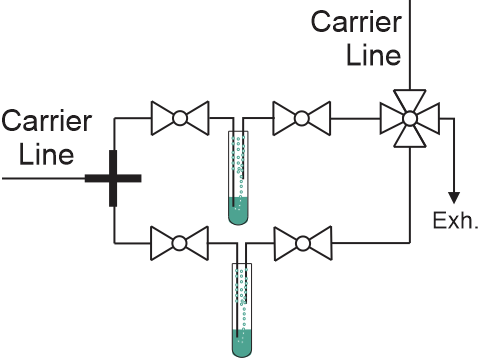
\includegraphics[width=0.5\textwidth,height=\textheight]{figures/ch9/multiplex-vapoursensor.png}

}

\caption{\label{fig-vapour-sensor-multiplexing}Multiplexing with a
second analyte bottle and four-way valve.}

\end{figure}



\end{document}
